\section{Theorie}
\label{sec:Theorie}

Die Ausbreitungsvorgänge elektromagnetischer Wellen lassen sich durch die Maxwellschen Gleichungen 
\begin{align*}
    \symup{rot}\, \vec{H} &= \vec{j} + \symup{\varepsilon \,\varepsilon_0}\,\dot{\vec{E}} \\
    \symup{rot}\, \vec{E} &= -\symup{\mu \, \mu_0} \,\dot{\vec{H}}
\end{align*}
beschreiben. Hier werden nicht-ferromagnetische und nicht elektrisch leitende Materialien betrachtet, wodurch $\mu \approx 1$ und
$\vec{j} = 0$ gilt. Der Poynting-Vektor
\begin{equation*}
    \vec{S} = \vec{E} \times \vec{H}
\end{equation*}
beschreibt die Strahlungsleistung pro Flächeneinheit. Mithilfe der Wellendarstellung des elektrischen und des magnetischen Feldes ergibt sich für 
den Betrag des Poynting-Vektors
\begin{equation}
    \lvert \vec{S} \rvert = v \,\symup{\varepsilon \,\varepsilon_0}\, \vec{E}^2 \; .
    \label{eqn:betragS}
\end{equation}

Wenn ein Lichtstrahl aus dem Vakuum unter dem Winkel $\alpha$ auf eine Grenzfläche fällt, wird ein Bruchteil des Lichts reflektiert. Der übrige 
Teil dringt in das Medium ein. Im Medium ist die Lichtgeschwindigkeit $v$ geringer als die Lichtgeschwindigkeit c. Dadurch erfährt der eindringende 
Lichtstrahl eine Richtungsänderung mit dem Brechungswinkel $\symup{\beta} < \symup{\alpha}$. Es ergibt sich eine Querschnittsänderung des 
Strahlenbündels. Der Energiesatz ergibt sich bei nicht absorbierenden Medien zu 
\begin{equation*}
    \symup{S_eF_e} = \symup{S_rF_e} + \symup{S_dF_d}
\end{equation*}
oder
\begin{equation*}
    \symup{S_ecos} \,\alpha = \symup{S_rcos} \,\alpha + \symup{S_dcos} \,\beta \; . 
\end{equation*}
Mit \autoref{eqn:betragS} ergibt dieser sich zu 
\begin{equation}
    \symup{c\varepsilon_0}{\vec{E_e}}^2\symup{cos} \,\alpha = \symup{c\varepsilon_0}{\vec{E_r}}^2\symup{cos} \,\alpha + v{\varepsilon \varepsilon_0}{\vec{E_d}}^2\symup{cos} \,\beta \; .
    \label{eqn:strahlung2}
\end{equation}
Desweiteren gelten für den Brechungsindex
\begin{equation*}
    \symup{n} = \frac{\symup{c}}{v}
\end{equation*}
und die Maxwellsche Relation
\begin{equation*}
    \symup{n}^2 = \symup{\varepsilon} \; .
\end{equation*}
Damit lässt sich $\varepsilon$ in \autoref{eqn:strahlung2} eliminieren und es ergibt sich
\begin{equation}
    \left({\vec{E_e}}^2-{\vec{E_r}}^2\right)\symup{cos} \,\alpha = \symup{n}\,{\vec{E_d}}^2\symup{cos} \,\beta \; .
    \label{eqn:strahlung3}
\end{equation}

An dieser Stelle ist nun eine Fallunterscheidung notwendig, da die Polarisationsrichtung des Lichts relativ zur Einfallsebene, welche durch 
den einfallenden und den reflektierten Strahl aufgespannt wird, einen Einfluss auf die Messung hat. Entsprechend 
wird $\vec{E_e}$ in seine Komponenten zerlegt
\begin{equation*}
    \vec{E_e} = \vec{E_{\perp}} + \vec{E_{\|}} \; .
\end{equation*}

Es wird zuerst die Polarisation senkrecht zur Einfallsebene betrachtet. Dabei schwingt $\vec{E_{\perp}}$ tangential zur Grenzfläche. Dies ist in 
\autoref{fig:sPol} dargestellt. 
\begin{figure}
    \centering
    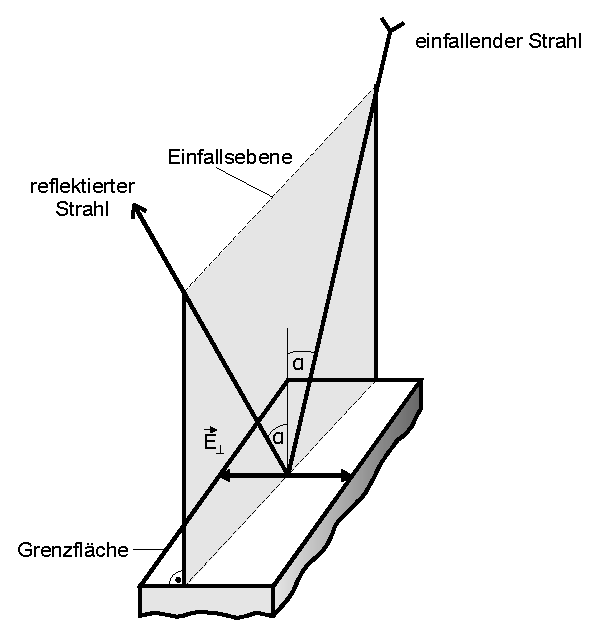
\includegraphics[height = 6cm]{sPol.pdf}
    \caption{Reflexion eines s-polarisierten Lichtstrahls an einer Grenzfläche \cite{ap407}.}
    \label{fig:sPol}
\end{figure}
Da das Linienintegral einer geschlossenen Kurve verschwindet, ist die Tangentialkomponente des Feldstärkevektors stetig. Daraus ergibt sich
\begin{equation*}
    \vec{E}_{\symup{e}_{\perp}} + \vec{E}_{\symup{r}_{\perp}} = \vec{E}_{\symup{d}_{\perp}} \; .
\end{equation*}
Aus dieser Stetigkeitsbedingung vereinfacht sich \autoref{eqn:strahlung3} zu 
\begin{equation*}
    \vec{E}_{\symup{r}_{\perp}} = - \vec{E}_{\symup{e}_{\perp}} \frac{\symup{ncos}\,\beta - \symup{cos}\,\alpha}{\symup{ncos}\,\beta + \symup{cos}\,\alpha} \; .
\end{equation*}
Mithilfe des Snelliusschen Brechungsgesetzes
\begin{equation*}
    \symup{n} = \frac{\symup{sin}\, \alpha}{\symup{sin}\, \beta}
\end{equation*}
erhält man die Fresnelschen Gleichungen 
\begin{equation*}
    \vec{E}_{\symup{r}_{\perp}} = - \vec{E}_{\symup{e}_{\perp}} \frac{\symup{sin}\left(\alpha - \beta\right)}{\symup{sin}\left(\alpha + \beta\right)}
\end{equation*}
und
\begin{equation}
    \vec{E}_{\symup{r}_{\perp}} = - \vec{E}_{\symup{e}_{\perp}} \frac{\left(\sqrt{\symup{n}^2-\symup{sin}^2 \, \alpha}-\symup{cos}\, \alpha\right)^2}{\symup{n}^2 - 1} \; .
    \label{eqn:fresnelS2}
\end{equation}
Wenn man \autoref{eqn:fresnelS2} nach n auflöst, erhält man
\begin{equation}
    n = \sqrt{1-\frac{4\vec{E}_{\symup{e}_{\perp}}\symup{cos}^2\, \alpha}{\left(\vec{E}_{\symup{r}_{\perp}}+\vec{E}_{\symup{e}_{\perp}}\right)^2}+\frac{4\vec{E}_{\symup{e}_{\perp}}\symup{cos}^2\, \alpha}{\vec{E}_{\symup{r}_{\perp}}+\vec{E}_{\symup{e}_{\perp}}}} \; .
    \label{eqn: n1}
\end{equation}

Nun wird die parallele Polarisationsrichtung betrachtet. Dabei schwingt $\vec{E}_{\|}$ in der Einfallsebene. Dies ist in \autoref{fig:pPol} dargestellt.
\begin{figure}
    \centering
    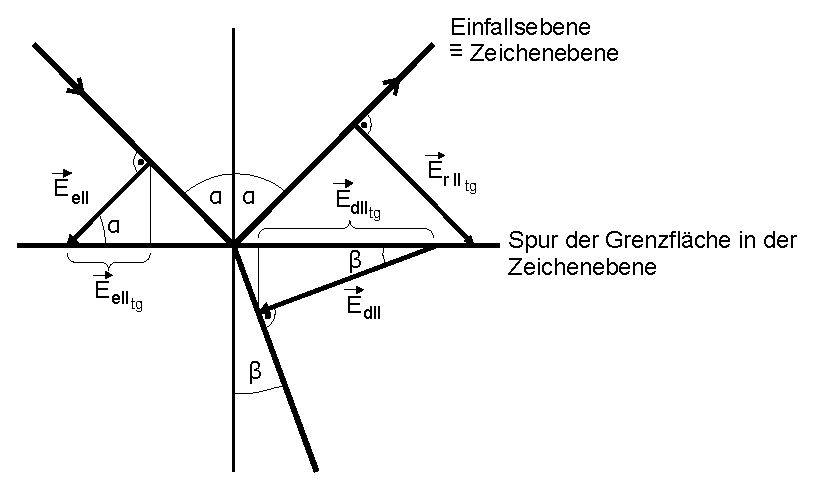
\includegraphics[height = 6cm]{pPol.pdf}
    \caption{Reflexion eines p-polarisierten Lichtstrahls an einer Grenzfläche \cite{ap407}.}
    \label{fig:pPol}
\end{figure}
$\vec{E}_{\|}$ besteht aus einer tangentialen Komponente $\vec{E}_{\| \symup{tg}}$ und einer normalen Komponente. Damit ergibt sich die Stetigkeitsbedingung 
\begin{equation*}
    \vec{E}_{\symup{e}\|\symup{tg}} + \vec{E}_{\symup{r}\|\symup{tg}} = \vec{E}_{\symup{d}\|\symup{tg}} \; .
\end{equation*}
Daraus folgt dann
\begin{equation*}
    \vec{E}_{\symup{r}\|} = \vec{E}_{\symup{e}\|} \frac{\symup{ncos}\, \alpha- \symup{cos}\, \beta}{\symup{ncos}\, \alpha + \symup{cos}\,\beta} \; .
\end{equation*}
Es ergeben sich mit dem Snelliusschen Brechungsgesetz weitere Fresnelsche Gleichungen
\begin{equation}
    \vec{E}_{\symup{r}\|} = - \vec{E}_{\symup{e}\|} \frac{\symup{tan}\left(\alpha - \beta\right)}{\symup{tan}\left(\alpha + \beta\right)}
    \label{eqn:fresnelP1}
\end{equation}
und
\begin{equation}
    \vec{E}_{\symup{r}\|} = \vec{E}_{\symup{e}\|}\frac{\symup{n}^2\symup{cos}\, \alpha - \sqrt{\symup{n}^2-\symup{sin}^2\,\alpha}}{\symup{n}^2\symup{cos}\, \alpha + \sqrt{\symup{n}^2-\symup{sin}^2\,\alpha}} \; .
    \label{eqn:fresnelP2}
\end{equation}
Auch diesmal kann \autoref{eqn:fresnelP2} nach n aufgelöst werden
\begin{equation*}
    n = \sqrt{\frac{1}{2}\left(\frac{\vec{E}_{\symup{r}\|}+\vec{E}_{\symup{e}\|}}{\vec{E}_{\symup{r}\|}-\vec{E}_{\symup{e}\|}}\frac{1}{\symup{cos}\,\alpha}\right)^2 \pm 
    \sqrt{\frac{1}{4}\left(\frac{\vec{E}_{\symup{r}\|}+\vec{E}_{\symup{e}\|}}{\vec{E}_{\symup{r}\|}-\vec{E}_{\symup{e}\|}}\frac{1}{\symup{cos}\,\alpha}\right)^4 - 
    \left(\frac{\vec{E}_{\symup{r}\|}+\vec{E}_{\symup{e}\|}}{\vec{E}_{\symup{r}\|}-\vec{E}_{\symup{e}\|}}\right)^2 \symup{tan}^2\, \alpha}} \; .
\end{equation*}
Mit \autoref{eqn:fresnelP1} wird $\vec{E}_{\symup{r}\|} = 0$ für $\alpha_{\symup{p}}+\beta_{\symup{p}} = 90°$. Mit dem Snelliusschen Brechungsgesetz
folgt dann für den Brewsterwinkel $\alpha_{\symup{p}}$
\begin{equation*}
    \symup{tan}\,\alpha_{\symup{p}} = \symup{n} \; . 
\end{equation*}
Der Brewsterwinkel beschreibt den Einfallswinkel, bei dem der Lichtstrahl nicht mehr reflektiert wird, sondern vollständig in das Medium eindringt.